\section{Bethe Heitler events}
\label{ref:mcbethe}
As a check for the cuts applied in Section \ref{sec:bethe} to remove the elastic radiative tail, 
and to verify that the $\pi^0$s lost with those cuts are properly taken into account, 
the same cuts are applied to the MonteCarlo simulation. Elastic events with radiative
tail were generated and combined with the MonteCarlo $\pi^0$ events.

The cut described in \F{fig:bh_phi_mm} is reproduced in \F{fig:bethe_gsim} for the MonteCarlo.
A good agreement is found for the resolution in each $W$ bin and the spread and position of the elastic
radiative tail.




\begin{figure}[h]
 \begin{center}
 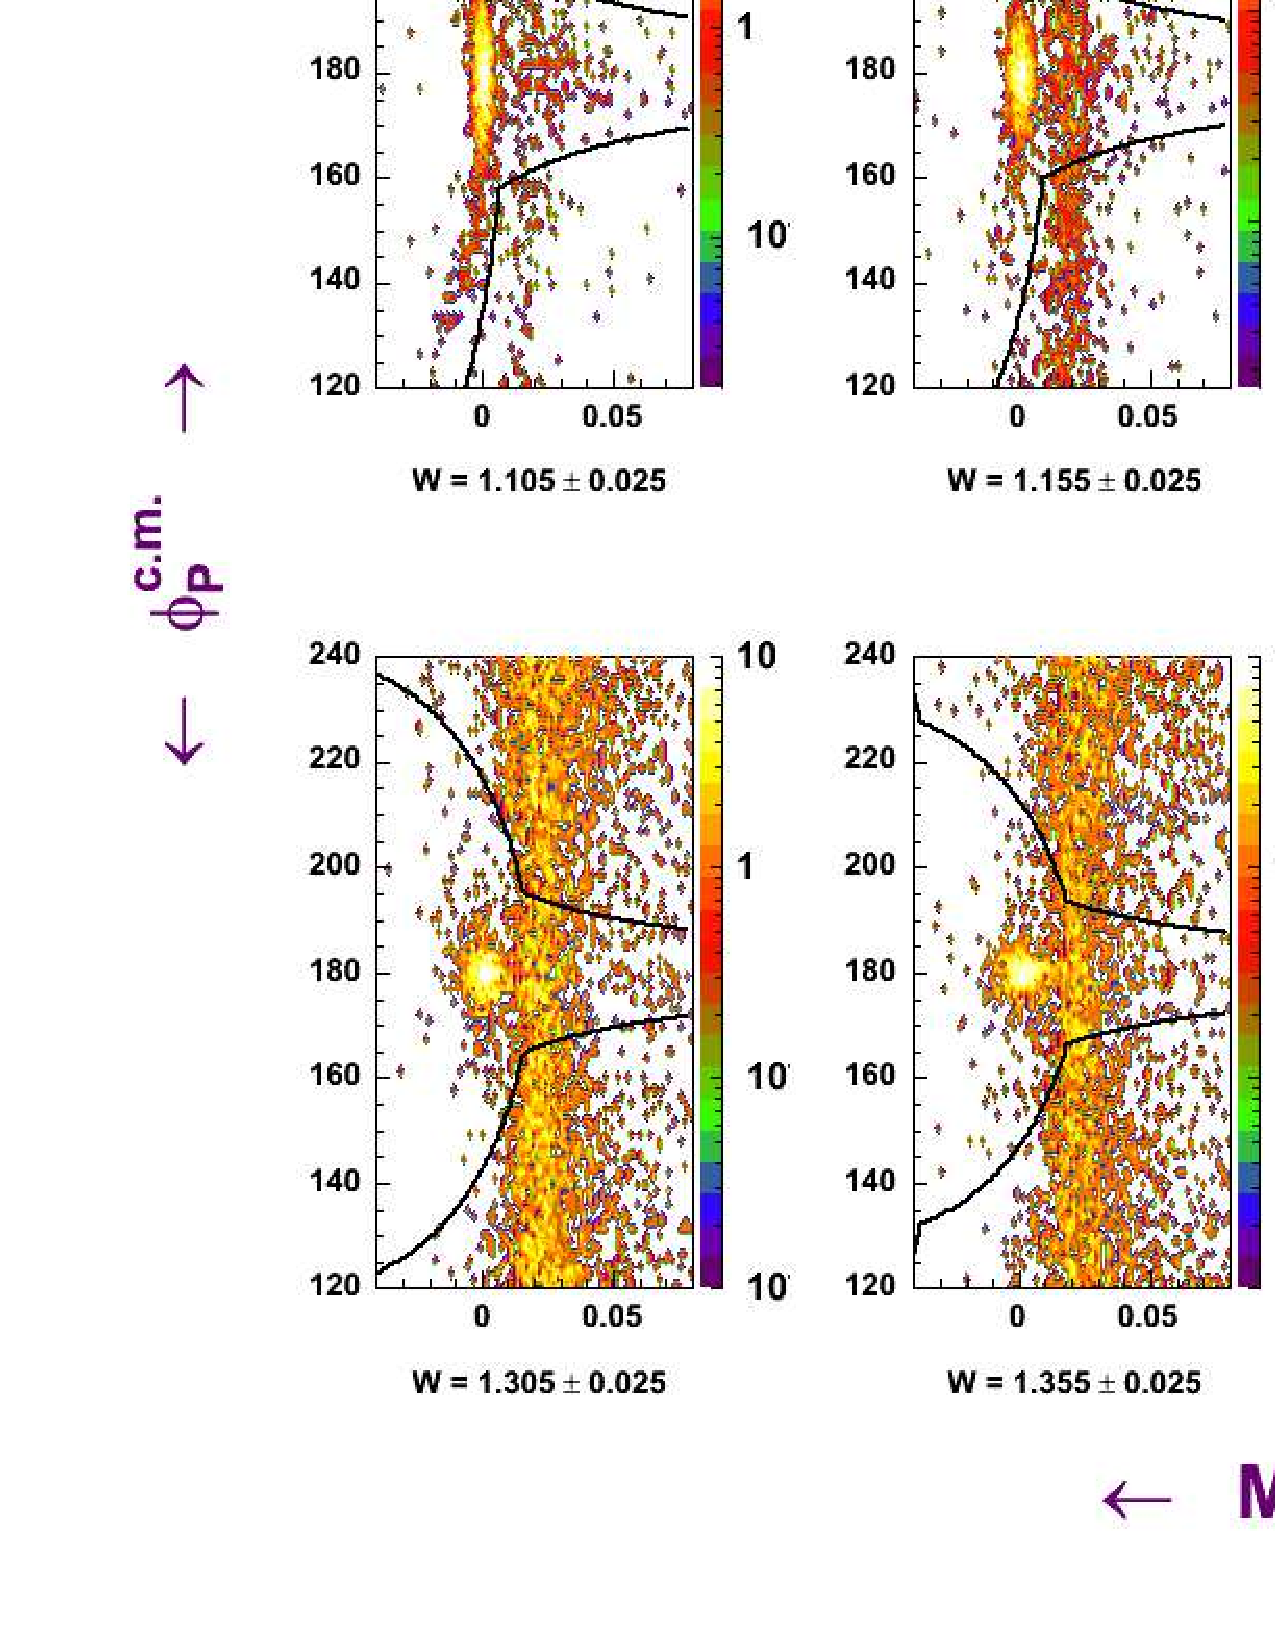
\includegraphics[width = 15.2cm, bb=40 40 1220 980]{acceptance/img/PHMMM} 
  \caption[$\phi_P^{c.m.}$ versus missing mass $M_x^2$ for different $W$ values for the MonteCarlo events]
          { $\phi_P^{c.m.}$ versus missing mass $M_x^2$ for different $W$ values for  
	             the MonteCarlo events. Good agreement with the data plotted in \F{fig:bh_phi_mm} 
		     is found.}
 \label{fig:bethe_gsim}
 \end{center}
\end{figure}


\cia

In \F{fig:mmw_gsim} is shown the missing mass $M_x^2$ spectra for data and MonteCarlo.
One can see $\pi^0$ events lost in the data with the Bethe-Heitler cuts are also lost in the MonteCarlo
so that they will be recovered with the acceptance calculation.     

\begin{figure}[h]
 \begin{center}
 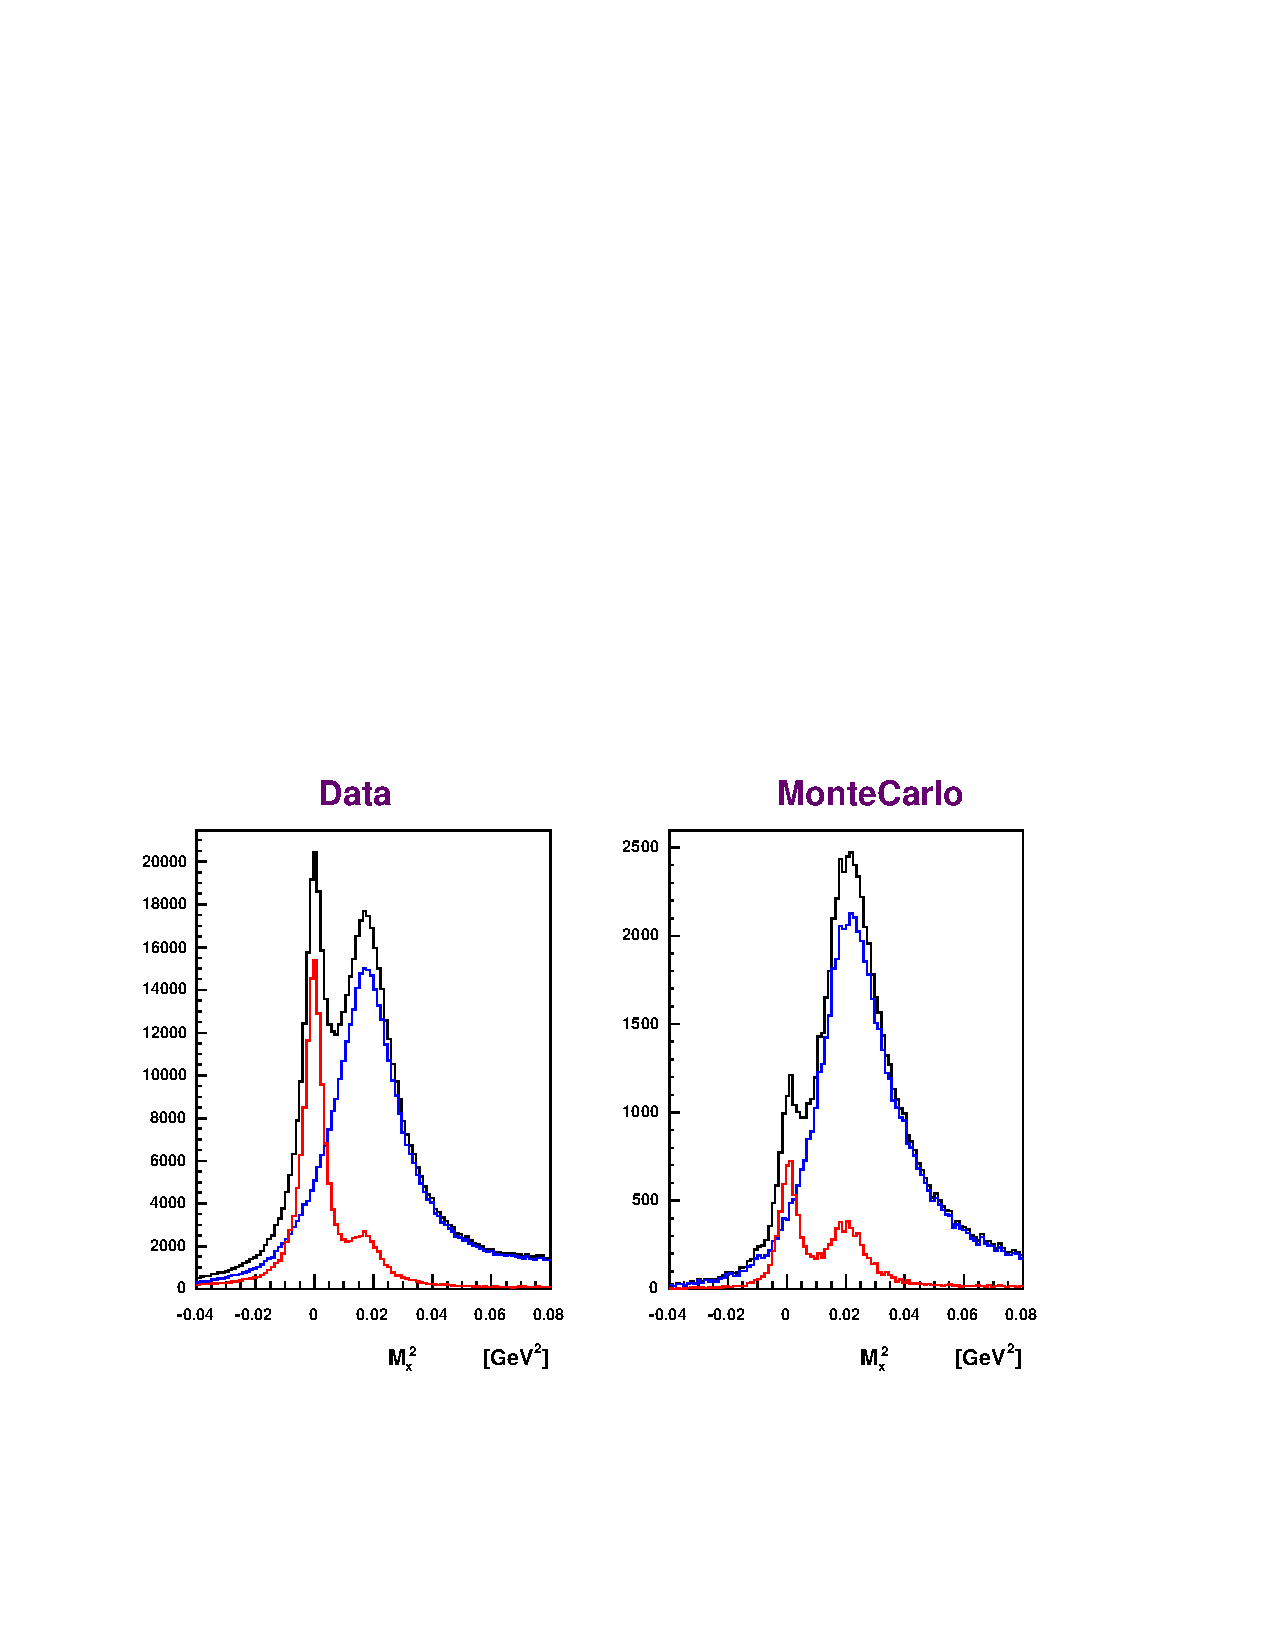
\includegraphics[width = 15.2cm, bb=20 100 560 500]{acceptance/img/MMW} 
  \caption[Missing mass $M_x^2$ spectra for data and MonteCarlo]
          { Missing mass $M_x^2$ spectra for data (left) and MonteCarlo (right).
	             $\pi^0$ events lost in the data with the Bethe-Heitler cuts
		     are also lost in the MonteCarlo.}
 \label{fig:mmw_gsim}
 \end{center}
\end{figure}

\cia\vspace{-2cm}
\section{Comparison between data and MonteCarlo}
A final check on the quality of the MonteCarlo simulation is shown in \F{fig:mm_gsim}
 where the missing mass $M_x^2$ spectra 
%and the $\phi^*$ distributions
is plotted for different values of kinematic variables. A good agreement is found between
data and MonteCarlo for the whole range of $W$ and $Q^2$.

\begin{figure}[h]
 \begin{center}
 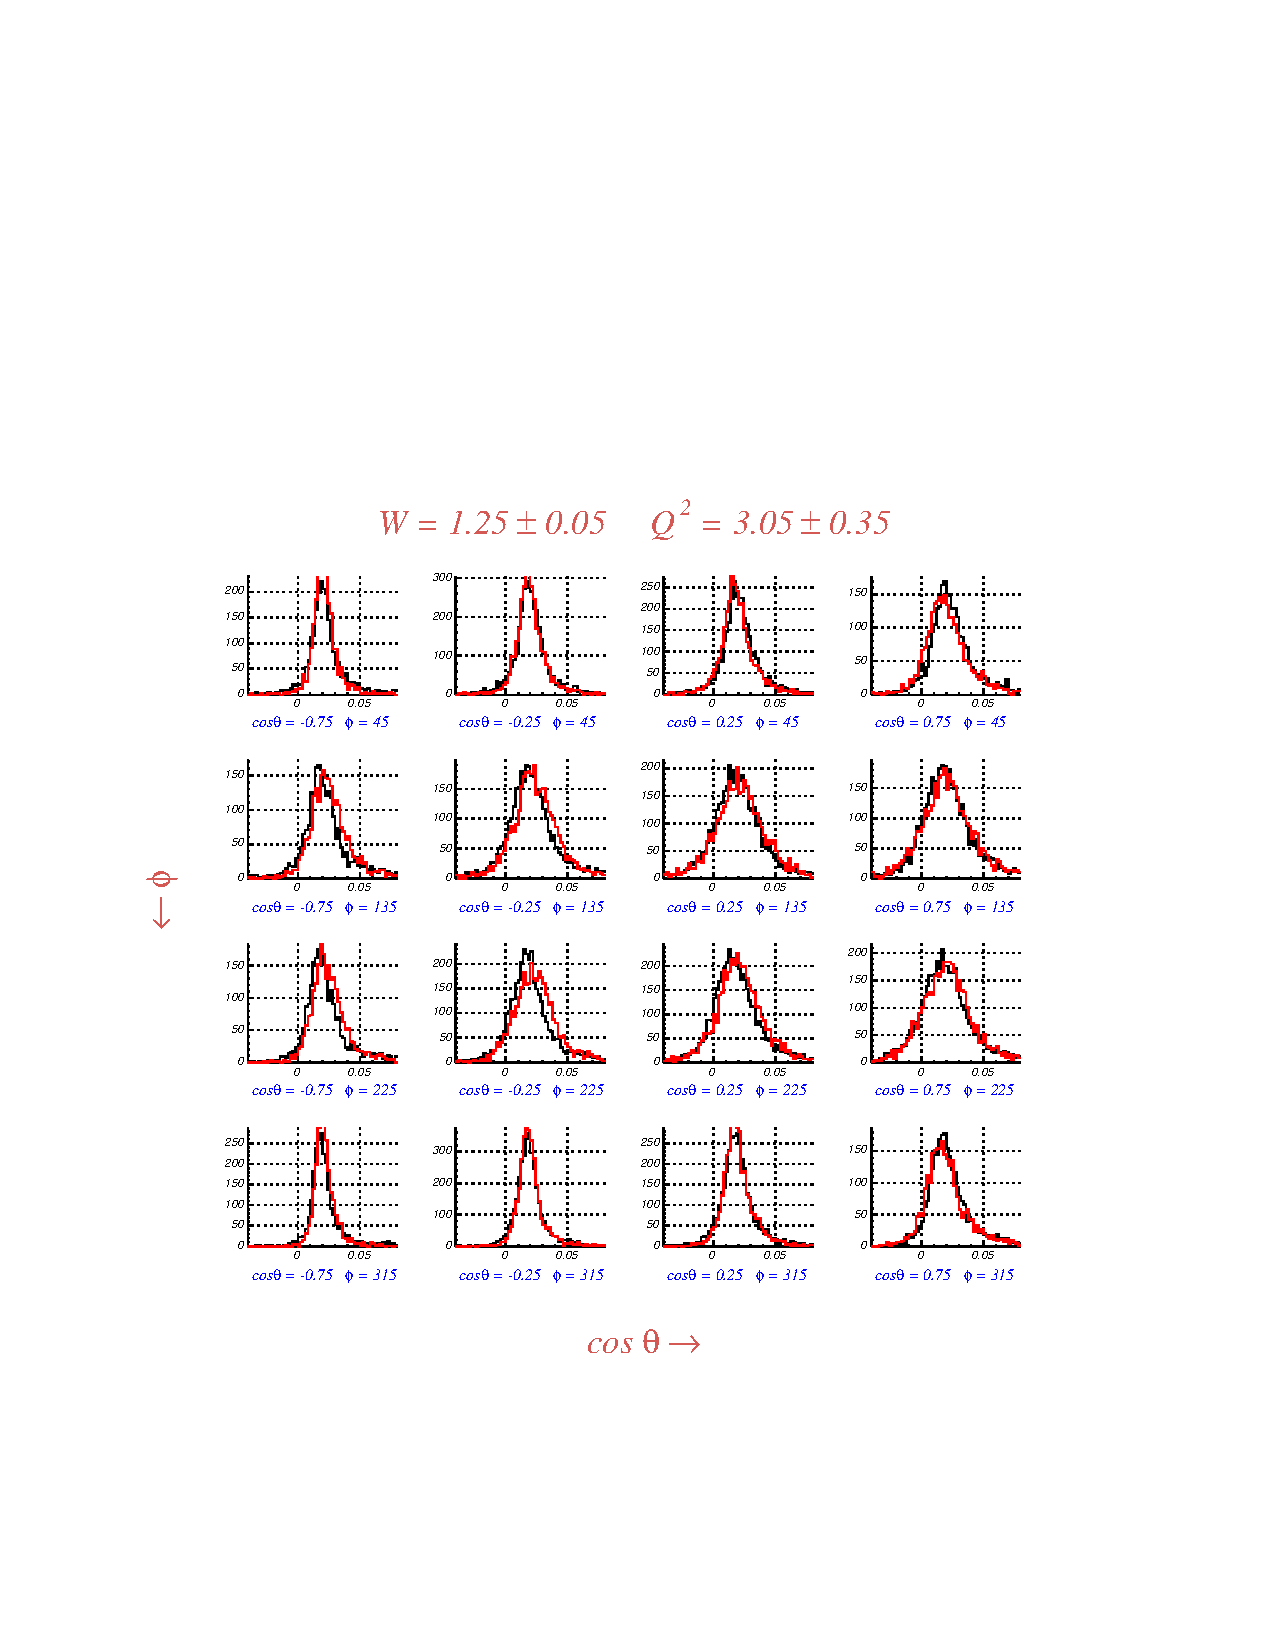
\includegraphics[width = 15.2cm, bb=60 120 520 560]{acceptance/img/comp_mm_datamc} 
  \caption[Missing mass $M_x^2$ spectra for data and MonteCarlo ]
          { Missing mass $M_x^2$ spectra for data (black) and MonteCarlo (red) for 
	             $1.2 < W < 1.3$, $Q^2 = 3.05\pm 0.35$ and different $\phi^*$, $\cos\theta^*$
		     values. A good agreement for mean position and resolution in different region of phase
		     space is found. }
 \label{fig:mm_gsim}
 \end{center}
\end{figure}

% \begin{figure}[h]
%  \begin{center}
%  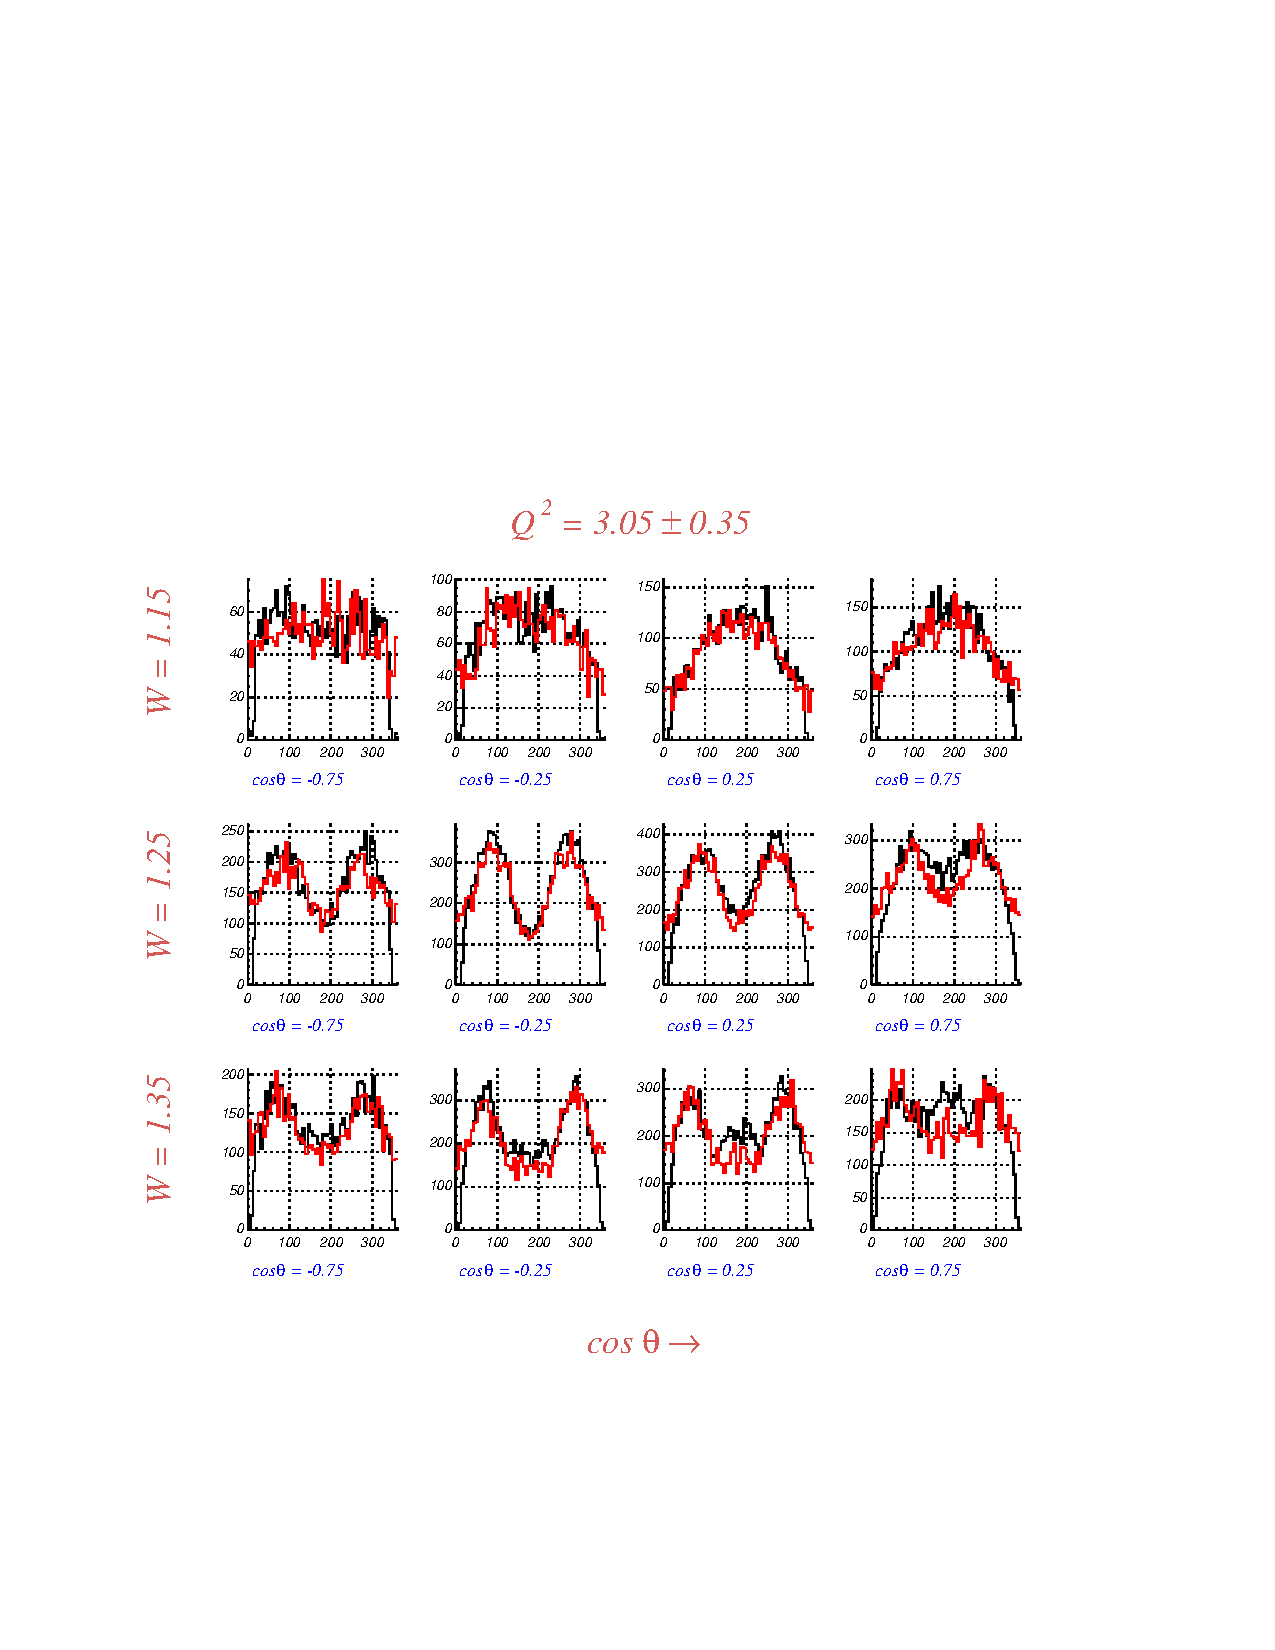
\includegraphics[width = 15.2cm, bb=60 100 520 600]{acceptance/img/comp_phi_datamc} 
%   \caption[ $\phi^*$ distributions for data and MonteCarlo]
%           { $\phi^*$ distributions for data (black) and MonteCarlo (red) for 
% 	             $Q^2 = 3.05\pm 0.35$ and different $W$, $\cos\theta^*$
% 		     values. A good agreement for mean position and resolution in different region of phase
% 		     space is found.  }
%  \label{fig:phi_gsim}
%  \end{center}
% \end{figure}
See    \begin{verbatim} 
        http://www.jlab.org/~ungaro/pi0eprod/com_phi 
        http://www.jlab.org/~ungaro/pi0eprod/com_miss
        http://www.jlab.org/~ungaro/pi0eprod/com_costh
\end{verbatim}
for a bin by bin comparison of the $\phi^*$, $\cos\theta^*$, missing mass $M_x^2$ between data
and MonteCarlo distributions.


